\section{Propulsion Motor}
The purpose of this block is to propel the vehicle forward by turning electrical energy into rotational energy. The propulsion motor is a DC-motor from Maxon Motors. 

\subsection{Analysis}
The motor under use in this project is a Maxon produced motor, article number 370355 \cite{DC-Motor}

The DC-motor in use, is actually a 36V motor, but due to the findings of the bachelor projekt "M7BAC\_Optimering af drivlinje", it is driven at overvoltage of 48V, which increases the motors efficiency. The motor in use is specified to run at 200W.\\
The motor has been modified to be able to fit inside the chassis. The modifications are length reductions to the rotating shaft. The reductions has no implications other than visuals. 

According to the datasheet, the motor has an efficiency of 94\% percent at most. This is the theoretical highest efficiency that should be improved even more as an effect of the overvoltage it is being driven at. 

The figure \vref{fig:DC-motor} shows the operating range of the motor in use. It shows how to control the motor and how the current consumption varies at different RPMs.

\begin{figure}[H]
	\centering
	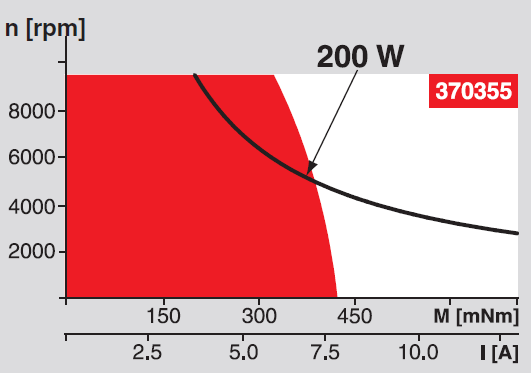
\includegraphics[width=0.6\linewidth]{Hardware/Pictures/DC-motor_diagram}
	\caption{Operating range of DC-motor in use}
	\label{fig:DC-motor}
\end{figure}

For full information concerning the motor, please refer to the datasheet.

For more information and test-resulst please refer to the documentation named "M7BAC\_Optimering af drivlinje"\cite{BAC_zenith33}. This document contains a thorough analysis of the motor in use and generally the propulsion system in use with on the vehicle.  

\subsection{Unity test}
The most critical parameter for the motor is the efficiency that it is able to be driven at. This efficiency would be able to be tested on Rolling-Road. This has not been completed in time for this Hand-in and therefore it is not possible to comment on the validity of the datasheet numbers. This test is expected to be completed before going to London as it is crucical information. 

To test the motor it must be set up to run directly on the generator on Rolling Road. The mounting for the motor alone is not completed and therefore the test is not possible. The reason for the remodelling of Rolling Road, is that in its current state its measures the efficiency of the entire driving system including the transmission and such. As neither of these are 100\% efficient the efficiency outputs cannot be validated. 